
\documentclass[border=8pt, multi, tikz]{standalone} 
\usepackage{import}
\subimport{../../layers/}{init}
\usetikzlibrary{positioning}
\usetikzlibrary{3d} %for including external image 

\def\ConvColor{rgb:yellow,5;red,2.5;white,5}
\def\ConvReluColor{rgb:yellow,5;red,5;white,5}
\def\PoolColor{rgb:red,1;black,0.3}
\def\UnpoolColor{rgb:blue,2;green,1;black,0.3}
\def\FcColor{rgb:blue,5;red,2.5;white,5}
\def\FcReluColor{rgb:blue,5;red,5;white,4}
\def\SoftmaxColor{rgb:magenta,5;black,7}   
\def\SumColor{rgb:blue,5;green,15}

\newcommand{\copymidarrow}{\tikz \draw[-Stealth,line width=0.8mm,draw={rgb:blue,4;red,1;green,1;black,3}] (-0.3,0) -- ++(0.3,0);}

\begin{document}
\begin{tikzpicture}
\tikzstyle{connection}=[ultra thick,every node/.style={sloped,allow upside down},draw=\edgecolor,opacity=0.7]
\tikzstyle{copyconnection}=[ultra thick,every node/.style={sloped,allow upside down},draw={rgb:blue,4;red,1;green,1;black,3},opacity=0.7]

\node[canvas is zy plane at x=0] (input) at (-3,0,0) {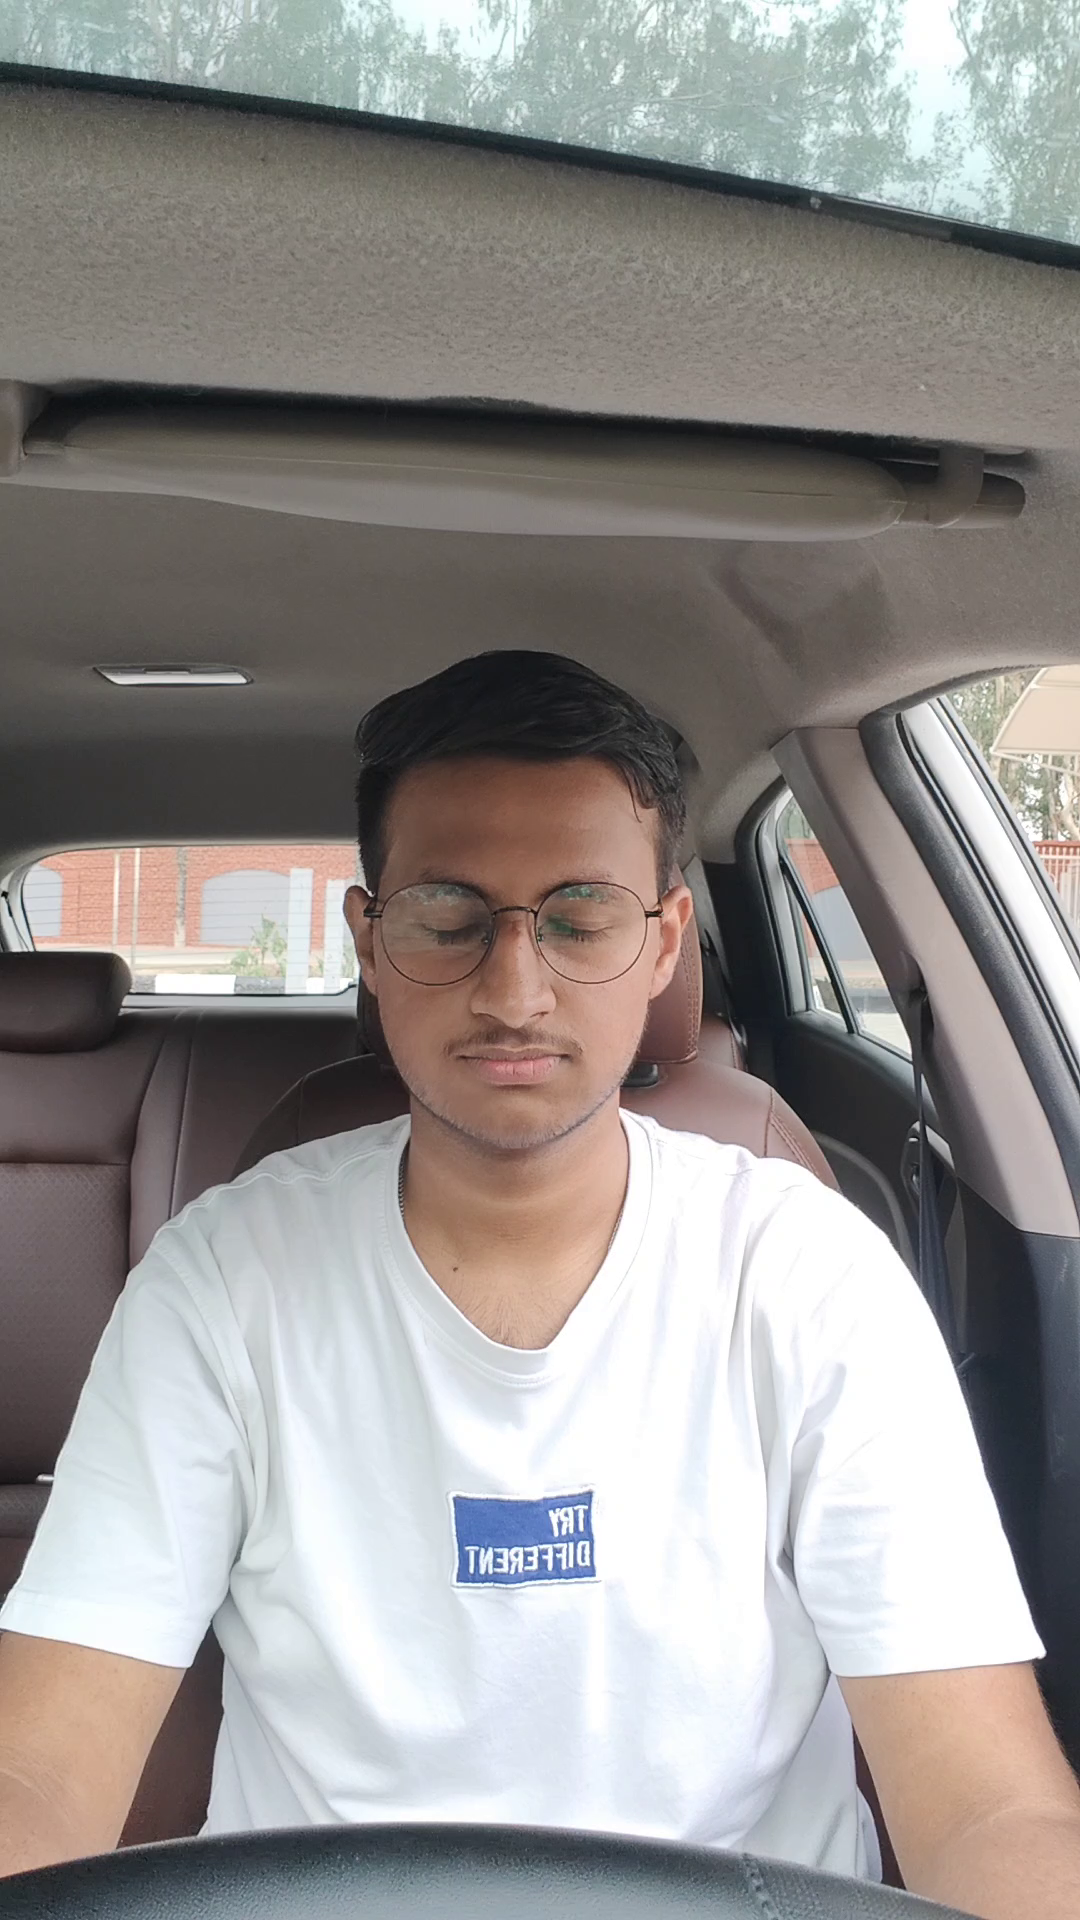
\includegraphics[width=8cm,height=8cm]{drowsy.png}};

\pic[shift={ (0,0,0) }] at (0,0,0) 
    {RightBandedBox={
        name=conv1,
        caption= ,
        xlabel={{ 64, 64 }},
        zlabel=224,
        fill=\ConvColor,
        bandfill=\ConvReluColor,
        height=40,
        width={ 2 , 2 },
        depth=40
        }
    };

\pic[shift={ (0,0,0) }] at (conv1-east) 
    {Box={
        name=pool1,
        caption= ,
        fill=\PoolColor,
        opacity=0.5,
        height=20,
        width=1,
        depth=20
        }
    };

\pic[shift={(1,0,0)}] at (pool1-east) 
    {Box={
        name=res2_0,
        caption= ,
        xlabel={{(64, 64, 256), }},
        zlabel=56,
        fill=\ConvColor,
        height=32,
        width=3.5,
        depth=32
        }
    };

\draw [connection]  (pool1-east)    -- node {\midarrow} (res2_0-west);

\pic[shift={(1,0,0)}] at (res2_0-east) 
    {Box={
        name=res2_1,
        caption= ,
        xlabel={{(64, 64, 256), }},
        zlabel=56,
        fill=\ConvColor,
        height=32,
        width=3.5,
        depth=32
        }
    };

\draw [connection]  (res2_0-east)    -- node {\midarrow} (res2_1-west);

\pic[shift={(1,0,0)}] at (res2_1-east) 
    {Box={
        name=res2_out,
        caption= ,
        xlabel={{(64, 64, 256), }},
        zlabel=56,
        fill=\ConvColor,
        height=32,
        width=3.5,
        depth=32
        }
    };

\draw [connection]  (res2_1-east)    -- node {\midarrow} (res2_out-west);

\path (res2_1-southeast) -- (res2_1-northeast) coordinate[pos=1.25] (res2_1-top) ;
\path (res2_1-south)  -- (res2_1-north)  coordinate[pos=1.25] (res2_1-top) ;
\draw [copyconnection]  (res2_1-northeast)  
-- node {\copymidarrow}(res2_1-top)
-- node {\copymidarrow}(res2_1-top)
-- node {\copymidarrow} (res2_1-north);

\pic[shift={(1,0,0)}] at (res2_out-east) 
    {Box={
        name=res3_0,
        caption= ,
        xlabel={{(128, 128, 512), }},
        zlabel=28,
        fill=\ConvColor,
        height=25,
        width=4.5,
        depth=25
        }
    };

\draw [connection]  (res2_out-east)    -- node {\midarrow} (res3_0-west);

\pic[shift={(1,0,0)}] at (res3_0-east) 
    {Box={
        name=res3_1,
        caption= ,
        xlabel={{(128, 128, 512), }},
        zlabel=28,
        fill=\ConvColor,
        height=25,
        width=4.5,
        depth=25
        }
    };

\draw [connection]  (res3_0-east)    -- node {\midarrow} (res3_1-west);

\pic[shift={(1,0,0)}] at (res3_1-east) 
    {Box={
        name=res3_2,
        caption= ,
        xlabel={{(128, 128, 512), }},
        zlabel=28,
        fill=\ConvColor,
        height=25,
        width=4.5,
        depth=25
        }
    };

\draw [connection]  (res3_1-east)    -- node {\midarrow} (res3_2-west);

\pic[shift={(1,0,0)}] at (res3_2-east) 
    {Box={
        name=res3_out,
        caption= ,
        xlabel={{(128, 128, 512), }},
        zlabel=28,
        fill=\ConvColor,
        height=25,
        width=4.5,
        depth=25
        }
    };

\draw [connection]  (res3_2-east)    -- node {\midarrow} (res3_out-west);

\path (res3_1-southeast) -- (res3_1-northeast) coordinate[pos=1.25] (res3_1-top) ;
\path (res3_2-south)  -- (res3_2-north)  coordinate[pos=1.25] (res3_2-top) ;
\draw [copyconnection]  (res3_1-northeast)  
-- node {\copymidarrow}(res3_1-top)
-- node {\copymidarrow}(res3_2-top)
-- node {\copymidarrow} (res3_2-north);

\pic[shift={(1,0,0)}] at (res3_out-east) 
    {Box={
        name=res4_0,
        caption= ,
        xlabel={{(256, 256, 1024), }},
        zlabel=14,
        fill=\ConvColor,
        height=16,
        width=5.5,
        depth=16
        }
    };

\draw [connection]  (res3_out-east)    -- node {\midarrow} (res4_0-west);

\pic[shift={(1,0,0)}] at (res4_0-east) 
    {Box={
        name=res4_1,
        caption= ,
        xlabel={{(256, 256, 1024), }},
        zlabel=14,
        fill=\ConvColor,
        height=16,
        width=5.5,
        depth=16
        }
    };

\draw [connection]  (res4_0-east)    -- node {\midarrow} (res4_1-west);

\pic[shift={(1,0,0)}] at (res4_1-east) 
    {Box={
        name=res4_2,
        caption= ,
        xlabel={{(256, 256, 1024), }},
        zlabel=14,
        fill=\ConvColor,
        height=16,
        width=5.5,
        depth=16
        }
    };

\draw [connection]  (res4_1-east)    -- node {\midarrow} (res4_2-west);

\pic[shift={(1,0,0)}] at (res4_2-east) 
    {Box={
        name=res4_3,
        caption= ,
        xlabel={{(256, 256, 1024), }},
        zlabel=14,
        fill=\ConvColor,
        height=16,
        width=5.5,
        depth=16
        }
    };

\draw [connection]  (res4_2-east)    -- node {\midarrow} (res4_3-west);

\pic[shift={(1,0,0)}] at (res4_3-east) 
    {Box={
        name=res4_4,
        caption= ,
        xlabel={{(256, 256, 1024), }},
        zlabel=14,
        fill=\ConvColor,
        height=16,
        width=5.5,
        depth=16
        }
    };

\draw [connection]  (res4_3-east)    -- node {\midarrow} (res4_4-west);

\pic[shift={(1,0,0)}] at (res4_4-east) 
    {Box={
        name=res4_out,
        caption= ,
        xlabel={{(256, 256, 1024), }},
        zlabel=14,
        fill=\ConvColor,
        height=16,
        width=5.5,
        depth=16
        }
    };

\draw [connection]  (res4_4-east)    -- node {\midarrow} (res4_out-west);

\path (res4_1-southeast) -- (res4_1-northeast) coordinate[pos=1.25] (res4_1-top) ;
\path (res4_4-south)  -- (res4_4-north)  coordinate[pos=1.25] (res4_4-top) ;
\draw [copyconnection]  (res4_1-northeast)  
-- node {\copymidarrow}(res4_1-top)
-- node {\copymidarrow}(res4_4-top)
-- node {\copymidarrow} (res4_4-north);

\pic[shift={(1,0,0)}] at (res4_out-east) 
    {Box={
        name=res5_0,
        caption= ,
        xlabel={{(512, 512, 2048), }},
        zlabel=7,
        fill=\ConvColor,
        height=8,
        width=6.5,
        depth=8
        }
    };

\draw [connection]  (res4_out-east)    -- node {\midarrow} (res5_0-west);

\pic[shift={(1,0,0)}] at (res5_0-east) 
    {Box={
        name=res5_1,
        caption= ,
        xlabel={{(512, 512, 2048), }},
        zlabel=7,
        fill=\ConvColor,
        height=8,
        width=6.5,
        depth=8
        }
    };

\draw [connection]  (res5_0-east)    -- node {\midarrow} (res5_1-west);

\pic[shift={(1,0,0)}] at (res5_1-east) 
    {Box={
        name=res5_out,
        caption= ,
        xlabel={{(512, 512, 2048), }},
        zlabel=7,
        fill=\ConvColor,
        height=8,
        width=6.5,
        depth=8
        }
    };

\draw [connection]  (res5_1-east)    -- node {\midarrow} (res5_out-west);

\path (res5_1-southeast) -- (res5_1-northeast) coordinate[pos=1.25] (res5_1-top) ;
\path (res5_1-south)  -- (res5_1-north)  coordinate[pos=1.25] (res5_1-top) ;
\draw [copyconnection]  (res5_1-northeast)  
-- node {\copymidarrow}(res5_1-top)
-- node {\copymidarrow}(res5_1-top)
-- node {\copymidarrow} (res5_1-north);

\pic[shift={ (2,0,0) }] at (res5_out-east) 
    {Box={
        name=gap,
        caption=Global Avg Pool,
        fill=\PoolColor,
        opacity=0.5,
        height=1,
        width=1,
        depth=40
        }
    };

\draw [connection]  (res5_out-east)    -- node {\midarrow} (gap-west);

\pic[shift={(1,0,0)}] at (gap-east) 
    {Box={
        name=fc1,
        caption=Dense 1024,
        zlabel=1,
        fill=\SoftmaxColor,
        height=1,
        width=1,
        depth=30
        }
    };

\draw [connection]  (gap-east)    -- node {\midarrow} (fc1-west);

\pic[shift={(1,0,0)}] at (fc1-east) 
    {Box={
        name=fc2,
        caption=Dense Softmax,
        zlabel=1,
        fill=\SoftmaxColor,
        height=1,
        width=1,
        depth=20
        }
    };

\draw [connection]  (fc1-east)    -- node {\midarrow} (fc2-west);

\pic[shift={(1,0,0)}] at (fc2-east) 
    {Box={
        name=softmax,
        caption=Output,
        xlabel={{" ","dummy"}},
        zlabel=5,
        fill=\SoftmaxColor,
        opacity=0.8,
        height=3,
        width=1.5,
        depth=25
        }
    };

\draw [connection]  (fc2-east)    -- node {\midarrow} (softmax-west);

\end{tikzpicture}
\end{document}
